\documentclass[12pt]{article}
\usepackage{graphicx}
\usepackage{hyperref}
\usepackage[margin=1.25in]{geometry}
\usepackage[utf8]{inputenc}
\graphicspath{ {./Figures/} }
\hypersetup{
    colorlinks=true,
    linkcolor=blue,
    filecolor=magenta,      
    urlcolor=cyan,
}
\urlstyle{same}
\usepackage[font={small,it}]{caption}
\usepackage{fancyvrb}
\title{Regression Analysis of Chicago Crime Volume by Ward using Public School Data}
\author{John D. Bulger, Valparaiso University\thanks{``I have neither given or received, nor have I tolerated other’s use of unauthorized aid."}}
\date{October 5, 2018}

\begin{document}
	\pagenumbering{gobble}
\begin{titlepage}
	\maketitle
\end{titlepage}
	\pagenumbering{arabic}

	\section{Introduction}
	
Crime levels have been a disturbing and interesting topic for a large portion of the city's history.  Infamous criminals such as Al Capone, John Dillinger, and John Wayne Gacy made names for themselves through their ``work" in the Windy City.  Within the past decade or so, Chicago’s crime rate (and homicide rate in particular) has experienced a surge.  2016 was the deadliest year in recent memory for the city.  According to Time Magazine's analysis of public data, Chicago experienced 27.7 homicides per 100,000 people, a 10-point increase over 2015.  It also outpaced the homicide rates of New York, Los Angeles, and Houston.  Overall, all other types of crimes increase year-over-year for Chicago as well.\cite{sanburn}

\par

Many theories attempt to explain this spike in crime (often unsuccessfully), but this analysis will explore it through the lens of public high school data.  The city of Chicago maintains an open data portal.  Official crime data by year, as well as an abundance of school data, can be easily accessed and used for analysis.  Additionally, since this data is directly reported by city agencies, it is generally viewed to be more accurate when compared to pulling data directly from third parties, such as news articles.

\par

The crime data and school data can be linked geographically by ward.  The city of Chicago is divided into 50 wards, which function as political districts.  While wards are not as well-recognized or segmented as Chicago’s community areas (such as Lincoln Park and Logan Square), wards are adjusted after every census to ensure each ward consists of approximately the same population.  While this would detract from a time-series analysis (for which community areas may be the best choice), wards should act as an effective record for this cross-sectional analysis.

\par

This analysis will focus on crime rate as a function of independent variables identified from the school data for the 2016-2017 school year.  Only crimes that occur within these time constraints will be used in the creation of this regression.  While analysis may well extract only homicides, violent crimes, or other subsections of the total crime picture for deeper analysis, the principal analysis of this paper will focus on total crime count.  Since population of wards are approximately the same and 2016 has no concrete population data by ward, a count of crimes by ward will function as effectively as creating a crime-rate target.

	\section{Prior Work}

Researchers from all disciplines have sought to shed light on the driving force that leads to crime.  While many data mining methods are capable of exploring relationships between variables driving crime, regression remains on of the most widely accepted.\cite{kaur}  This is in part due to the clearly defined effects of the independent variables on the dependent variable, which is lacking in many state-of-the-art data science algorithms (known as ``black box algorithms").

\paragraph{Micro-Level}

Many instances of regression analysis on micro-level crime data have been explored and documented.  In light of the high school focus of this analysis, prior work centered on juvenile subjects is of utmost interest.  Alcohol abuse among juveniles is exhibits a statistically significant relationship with crime rates, leading researchers to suspect a possible causal effect.\cite{fergusson}  Relationships between nicotine dependence and cannabis abuse with crime have also be identified via regression analysis.\cite{ferg2}  Additionally, the association with ``deviant peers" was shown to have a significant effect on likelihood to commit a crime.  Deviant peers were measured as a scale score from the number of the subject's friends who engaged in substance abuse, received school discipline and suspensions, or who broke the law.  While the effect of peer deviation on crime likelihood appears to decrease as maturity is reached, it has a substantial effect during high school years.\cite{ferg2}

\par

A enlightening micro-level study by Azim Shariff and Mijke Rhemtulla used regression analysis to discover, in their samples, that beliefs in heaven and hell were the most influential independent variables in committing crimes, even when compared to more ``traditional" variables typically associated with crime.\cite{shariff}  The effects of the heaven and hell variables held true for a multitude of crimes, even when presented in a multivariate regression with common variables such as poverty level and amount of population incarcerated.  By evaluating the regression in this way, this study stands as a prime example of how some of the most influential variables could easily be overlooked.

\paragraph{Macro-Level}

Two examples of macro-level crime regression, ones that are very similar in nature to this analysis, focused on crime levels in Salinas, California.  The first paper, written in 2009, examines various socio-economic indicators as variables in a regression of violent crime.  These indicators included public school metrics, notably dropout rate, graduation rate, and attendance.  All of these metrics were found to have some level of relationship with crime levels.\cite{salinas_env}

\par

The second analysis built upon the previous study by taking different regression estimators (beyond OLS) and compared the results when modeled as a predictive algorithm.  In the best OLS estimate, included variables consisted of number of vacant home units, overpopulation percentage, unemployment, number of police, and police department budget.\cite{salinas_crime}  While these variables do not relate to public school data, as will be examined later, this stands as an excellent example and guide to modeling crime rates via OLS on a macro-level.

	\section{Data}


\subsection{Procurement \& Preprocessing}

All of the data used in this regression analysis is freely available at the city's Open Data Portal.\cite{c1data}\cite{c2data}\cite{s1data}\cite{s2data}\cite{s3data}  The school data consisted of different metrics and information spread over three data files.  These datasets were able to be merged by school ID.  High schools were then isolated, and the variables were averaged by ward.\footnote{Not all of the 50 wards contained a high school.  So while 50 wards exist, this research only takes 48 into account.}  Imputation by median value was conducted where necessary.

\par

The crime data was contained in two datasets from 2016 and 2017.  Each record was a reported instance of a crime and contained attributes regarding location, type of crime, UCR code, and other information.  The two years of data were combined; then, crimes that occurred outside of the 2016-2017 school year were dropped.  The total number of crimes, as well as the total number of homicides, were summed by ward.  The school data was then joined to the crime data by ward to create the final dataset used in this regression analysis.\footnote{This data preprocessing was conducted using R and Python.  Scripts and data can be found in the GitHub repository for this project at \href{https://github.com/jdbul33/reimagined-parakeet}{https://github.com/jdbul33/reimagined-parakeet}.}


\subsection{Variables}

\paragraph{Dependent Variables}
Relevant variables were chosen from this final dataset, upon which the regression will be built.  The two dependent variables were identified as total crime instances and total homicide count by ward for the 2016-2017 school year.  The basic statistical description of these variables can be seen in Table 1.

\begin{center}
	\begin{table}[h]
	\begin{tabular}{ c | c | c | c | c | c }
		
		 & \textbf{Mean} & \textbf{Median} & \textbf{Std. Dev.} & \textbf{Minimum} & \textbf{Maximum} \\ 
		 \hline
		 \textbf{Total Crime} & 4,194 & 3,280 & 2327 & 1,824 & 12,057 \\
		 \textbf{Homicides} & 12 & 7.5 & 11.7 & 0 & 45 \\
    
	\end{tabular}
\caption{Descriptive statistics of the dependent variables for Chicago by ward}
\end{table}
\end{center}  

\paragraph{Independent Variables}
Independent variables were then identified from the dataset, based on theory, prior work on this subject, and availability.  OLS necessitates that all variables used with the estimator must be stated numerically; therefore, all chosen variables are either numeric or able to be translated as such.\footnote{Dress Code is a dummy, binary variable.  Schools with a dress code are valued at 1, while those without a dress code are denoted by 0.  Therefore, each ward will have a dress code value of 0-1, depending on the mix of high schools in that ward.}\footnote{Survey variables result from surveys given to teachers and students to rank their school in five criteria:  supportive environment, involved families, school safety, collaborative teaching, and ambitious instruction.  Scoring is from 0-5 with 5 being the best.}  This precluded many free-format data fields consisting of comments or non-ordinal evaluation.  The chosen variables, and their descriptive statistics, can be seen in Table 2.  These consist of the initial variables that were evaluated for regression analysis, not the final model's variables.

\begin{center}
	\begin{table}[h]
		\begin{tabular}{ c | c | c | c | c | c }
			
			& \textbf{Mean} & \textbf{Median} & \textbf{Std. Dev.} & \textbf{Minimum} & \textbf{Maximum} \\ 
			\hline
			\textbf{Graduation Rate} & 72.9\% & 74.6\% & 13.7\% & 27.8\% & 93.5\% \\
			\textbf{College Enrollment} & 49.3\% & 50.2\% & 18.0\% & 10.8\% & 85.7\% \\
			\textbf{Dress Code} & 0.6 & 0.6 & 0.4 & 0 & 1\\
			\textbf{Average ACT Score} & 17.0 & 16.8 & 2.2 & 13.1 & 22.3\\
			\textbf{Survey-Supportive} & 3.3 & 3.4 & 0.7 & 1 & 5\\
			\textbf{Survey-Families} & 3.2 & 3.2 & 1 & 0 & 5\\
			\textbf{Survey-Safety} & 2.1 & 2 & 0.6 & 0.5 & 3.7\\
			\textbf{Survey-Teachers} & 3.5 & 3.5 & 0.9 & 0 & 5\\
			\textbf{Survey-Instruction} & 3.7 & 4 & 0.8 & 1.5 & 5\\
			\textbf{Student Attendance} & 85.5\% & 87.8\% & 7.6\% & 53.8\% & 95.4\% \\
			\textbf{Teacher Attendance} & 92.5\% & 92.6\% & 0.6\% & 91.1\% & 93.6\% \\
			\textbf{Suspensions/100 stud.} & 22.5 & 16.6 & 19 & 0.6 & 103\\
			\textbf{Dropout Rate} & 10.3\% & 7.2\% & 8.7\% & 0.9\% & 33.4\% \\
			\textbf{Low Income Students} & 85.5\% & 90.2\% & 10.8\% & 54.3\% & 95.7\% 
			
		\end{tabular}
		\caption{Descriptive statistics of candidate independent variables for Chicago high schools by ward}
	\end{table}
\end{center}

These candidate variables were then evaluated for multicollinearity, as correlated independent variables violate one of the basic assumptions of OLS.  This was completed visually (since the number of variables chosen was relatively small) utilizing R, a statistical software.  The resulting correlations can be seen in Figure 1.  This information was referenced as final variables were selected.

	\begin{figure}
		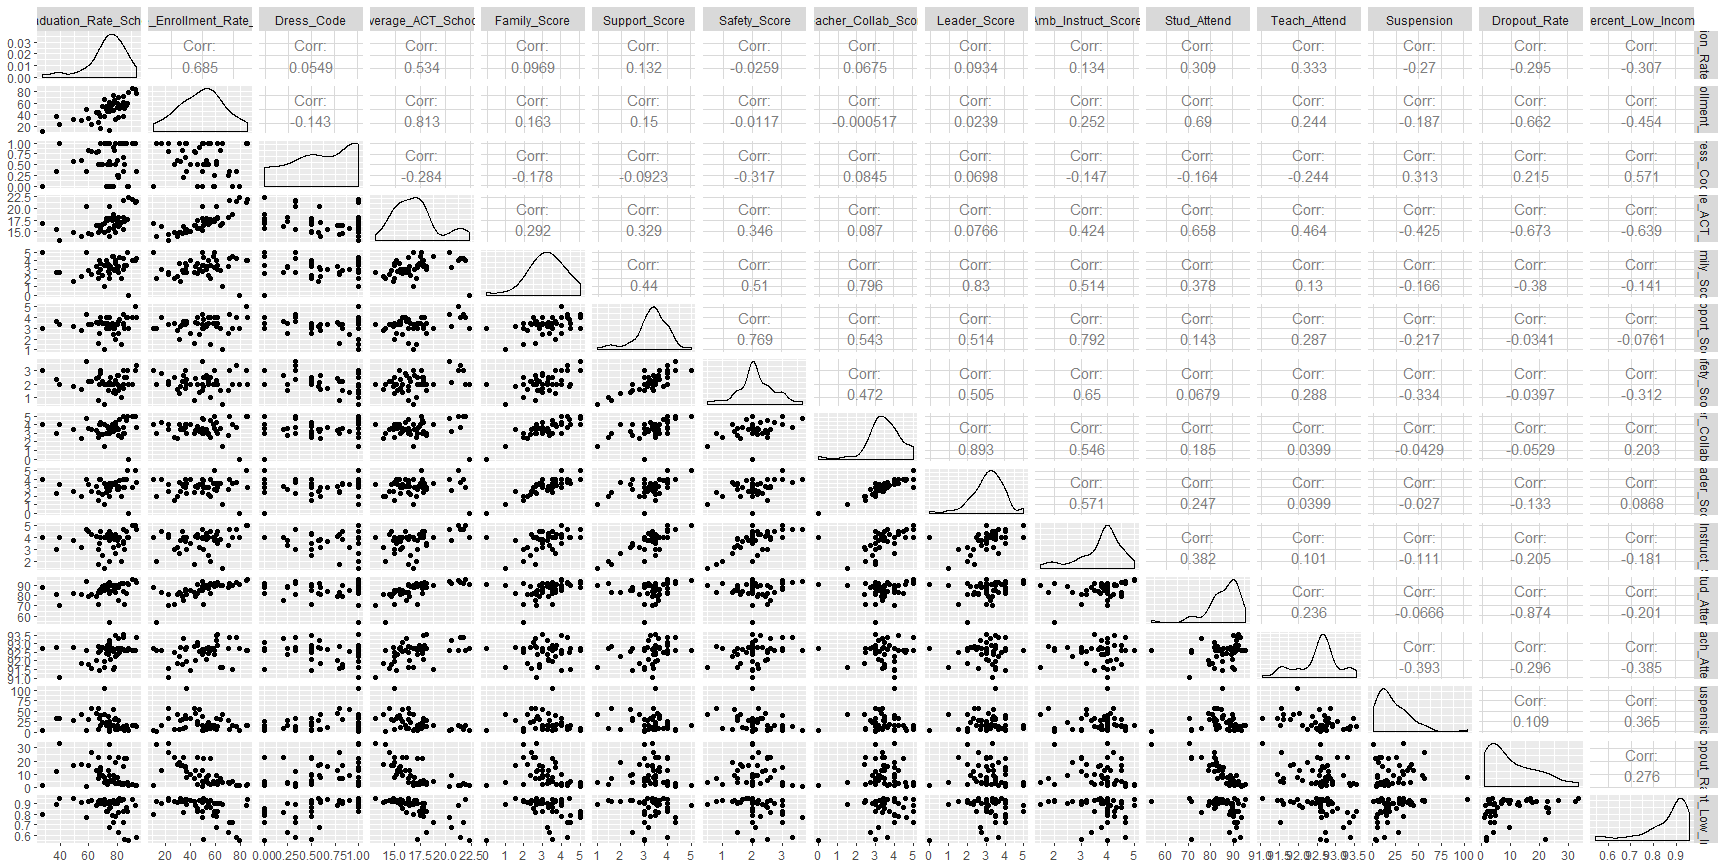
\includegraphics[scale=.33]{pairplot.png}
		\caption{Visualization of correlations and distributions of candidate independent variables}
	\end{figure}

\subsection{Model}

The model chosen to explain crime as a function of public school data was a linear regression, using Ordinary Least Squares as the estimator.  The variables shown in Table 2 represent all of the possible attributes from the data that could theoretically serve as a predictor and that could be coded in a numeric format, as explained earlier.  In order to narrow these variables into an initial model, stepwise regression was utilized.  This was conducted using R, with a separate analysis conducted for each of the dependent variables:  total crime and total homicides.  Once completed, these selected variables were tested for multicollinearity and heteroskedacity, analyzed as a regression in SAS, and then subsequently worked into the best possible linear regression given the data.

\paragraph{Total Crime}

The stepwise regression for this analysis used Total Crime as the dependent variable and all of the initial variables in Table 2 as a starting point.  After running this analysis, the independent variables detected as most important



\paragraph{Total Homicides}


	\section{Analysis}
	


	\section{Discussion}



	\section{Conclusions}


\subsection{Opportunities for Further Work}








	\newpage
	\begin{thebibliography}{12}
	
\bibitem{sanburn}
Sanburn, J. and Johnson, D. (2017, January). See Chicago's Deadly Year in 3 Charts. \textit{Time}. Retrieved from \href{http://time.com/4635049/chicago-murder-rate-homicides}{http://time.com/4635049/chicago-murder-rate-homicides}.

\bibitem{kaur}
Kaur, S. and Singh, W. (2017). Systematic review of crime data mining. \textit{International Journal of Advanced Research in Computer Science, 8}(5).

\bibitem{fergusson}
Fergusson, D.M. and Horwood, L.J. (2000). Alcohol abuse and crime: a fixed-effects regression analysis. \textit{Addiction, 95}(10), 1525-1536.

\bibitem{ferg2}
Fergusson, D.M., Swain-Campbell, N.R., and Horwood, L.J. (2002). Deviant peer affiliations, crime, and substance use: a fixed effects regression analysis. \textit{Journal of Abnormal Child Psychology, 30}(4), 419-430.

\bibitem{shariff}
Shariff, A.F. and Rhemtulla M. (2012). Divergent effects of beliefs in heaven and hell on national crime rates. \textit{PLoS ONE, 7}(6). \href{https://doi.org/10.1371/journal.pone.0039048}{https://doi.org/10.1371/journal.pone.0039048}.

\bibitem{salinas_env}
Clarke, J.A. and Onufer, T.L. (2009). Understanding environmental factors that affect violence in Salinas, California. \textit{Calhoun: The NPS Institutional Archive}. Retrieved from \href{http://hdl.handle.net/10945/4466}{http://hdl.handle.net/10945/4466}.

\bibitem{salinas_crime}
Shingleton, J.S. (2012). Crime trend prediction using regression models for Salinas, California. \textit{Calhoun: The NPS Institutional Archive}. Retrieved from \href{http://hdl.handle.net/10945/7416}{http://hdl.handle.net/10945/7416}.

\bibitem{c1data}
City of Chicago. (2018). \textit{Crimes - 2016}[Data file]. Retrieved from \href{https://data.cityofchicago.org}{https://data.cityofchicago.org}.

\bibitem{c2data}
City of Chicago. (2018). \textit{Crimes - 2017}[Data file]. Retrieved from \href{https://data.cityofchicago.org}{https://data.cityofchicago.org}.

\bibitem{s1data}
City of Chicago. (2018). \textit{Chicago-Public-Schools-School-Locations-SY1617}[Data file]. Retrieved from \href{https://data.cityofchicago.org}{https://data.cityofchicago.org}.

\bibitem{s2data}
City of Chicago. (2017). \textit{Chicago Public Schools - School Progress Reports SY1617}[Data file]. Retrieved from \href{https://data.cityofchicago.org}{https://data.cityofchicago.org}.

\bibitem{s3data}
City of Chicago. (2017). \textit{Chicago Public Schools - School Profile Information SY1617}[Data file]. Retrieved from \href{https://data.cityofchicago.org}{https://data.cityofchicago.org}.

	\end{thebibliography}

\end{document}